213. \begin{figure}[ht!]
\center{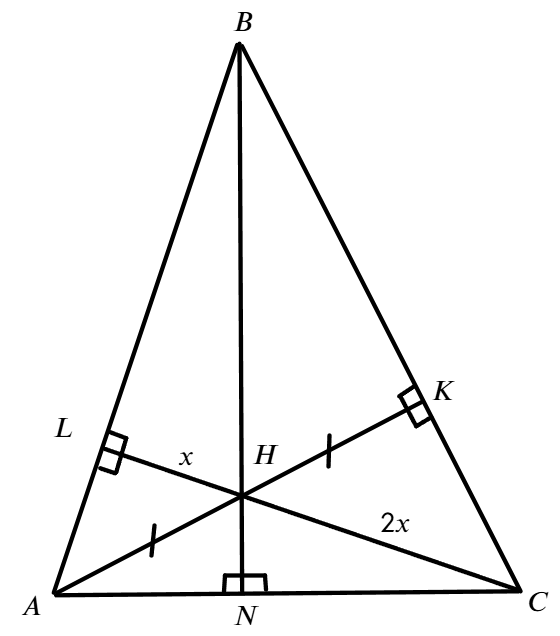
\includegraphics[scale=0.35]{g9-208.png}}
\end{figure}\\
Пусть  $HL=x,$ тогда $CH=2x.$ Треугольники $AHL$ и $CHK$ подобны по двум углам (углы $ALH$ и $CKH$ прямые, а $AHL$ и $CHK$ --- вертикальные), поэтому $\cfrac{AH}{CH}=\cfrac{LH}{HK},\ \cfrac{AH}{2x}=\cfrac{x}{AH},\ AH^2=2x^2,\ AH=HK=\sqrt{2}x.$ Тогда по теореме Пифагора для треугольника $ALH$ найдём $AL=\sqrt{AH^2-LH^2}=\sqrt{2x^2-x^2}=x.$ Треугольники $ALC$ и $ANB$ подобны по двум углам (углы $ANB$ и $ALC$ прямые, угол $A$ --- общий), поэтому
$\cfrac{CL}{BN}=\cfrac{AL}{AN},\ \cfrac{x+2x}{BN}=\cfrac{x}{AN},\ \cfrac{BN}{AN}=\cfrac{3x}{x}=3.$ Таким образом, $tg(\angle BAC)=\cfrac{BN}{AN}=3.$\\
